\documentclass[a4 paper]{article}
% Set target color model to RGB
\usepackage[inner=1.5cm,outer=1.5cm,top=2.5cm,bottom=2.5cm]{geometry}
\usepackage{setspace}
\usepackage[rgb]{xcolor}
\usepackage{verbatim}
\usepackage{amsgen,amsmath,amstext,amsbsy,amsopn,tikz,amssymb,tkz-linknodes}
\usepackage{fancyhdr}
\usepackage[colorlinks=true, urlcolor=blue,  linkcolor=blue, citecolor=blue]{hyperref}
\usepackage[colorinlistoftodos]{todonotes}
\usepackage{rotating}
\usepackage{enumitem}
\usepackage{amssymb}
\usepackage{graphicx}


%\usetikzlibrary{through,backgrounds}
\hypersetup{%
pdfauthor={Arman Shokrollahi},%
pdftitle={Homework},%
pdfkeywords={Tikz,latex,bootstrap,uncertaintes},%
pdfcreator={PDFLaTeX},%
pdfproducer={PDFLaTeX},%
}
%\usetikzlibrary{shadows}
\usepackage[francais]{babel}
\usepackage{booktabs}
\newcommand{\ra}[1]{\renewcommand{\arraystretch}{#1}}

      \newtheorem{thm}{Theorem}[section]
      \newtheorem{prop}[thm]{Proposition}
      \newtheorem{lem}[thm]{Lemma}
      \newtheorem{cor}[thm]{Corollary}
      \newtheorem{defn}[thm]{Definition}
      \newtheorem{rem}[thm]{Remark}
      \numberwithin{equation}{section}

\newcommand{\report}[5]{
   \pagestyle{myheadings}
   \thispagestyle{plain}
   \newpage
   \setcounter{page}{1}
   \noindent
   \begin{center}
   \framebox{
      \vbox{\vspace{2mm}
    \hbox to 6.50in { {\bf EC4213/ET5402/CT5303:~Machine learning and deep learning \hfill Fall 2019} }
       \vspace{4mm}
       \hbox to 6.28in { {\Large \hfill #1 \hfill}}
       \vspace{1mm}
       \hbox to 6.28in { {\hfill #2  \hfill} }
       \vspace{3mm}
       \hbox to 6.28in { {\it Instructor: #3 \hfill #4 (#5)}}
      \vspace{2mm}}
   }
   \end{center}
   \markboth{#5 -- #1}{#5 -- #1}
   \vspace*{4mm}
}

\newcommand{\bbF}{\mathbb{F}}
\newcommand{\bbX}{\mathbb{X}}
\newcommand{\bI}{\mathbf{I}}
\newcommand{\bX}{\mathbf{X}}
\newcommand{\bx}{\mathbf{x}}
\newcommand{\bY}{\mathbf{Y}}
\newcommand{\bw}{\mathbf{w}}
\newcommand{\bepsilon}{\boldsymbol{\epsilon}}
\newcommand{\balpha}{\boldsymbol{\alpha}}
\newcommand{\bbeta}{\boldsymbol{\beta}}
\newcommand{\0}{\mathbf{0}}
\DeclareMathOperator*{\argmax}{arg\,max}
\DeclareMathOperator*{\argmin}{arg\,min}
\newcommand\gldec[2]{
\underset{#1}{\overset{#2}{\gtrless}}
}
\usepackage{titlesec}
\titlespacing*{\section}
{1.5em}{1.5em}{1em}
\titlespacing*{\subsection}
{1.5em}{1em}{1em}


\begin{document}
\report{Report for CA2}{}{Jonghyun Choi}{Jisu Shin}{20175095}

REPORT1. \begin{figure}[h] 

\begin{center}


\includegraphics[width=1.0\linewidth]{vanila linear regression error.png}

\end{center}

\caption{error printed by vanila linear regression }

\label{fig:long}

\label{fig:onecol}

\end{figure}

Above figure shows the result error of the vanila linear regression I implemented. The error seems quite large but the given data size was also large so I think it is reasonable. To reduce the error, kernel can be used as it is mentioned, and also there are many kinds of input data, so finding the relationship on those data and handle those data differently will be helpful. Also to reduce error, we should prevent overfitting by set the limit of parameter w, or using the ridge regression, etc.

REPORT2. \begin{figure}[!h] 

\begin{center}

\includegraphics[width=0.3\linewidth]{Accuracy of the model as a function of the regularization.png}

\end{center}

\caption{Graph with x-axis : gamma, y-axis : accuracy}

\label{fig:long}

\label{fig:onecol}

\end{figure}

\begin{figure}
\begin{center}

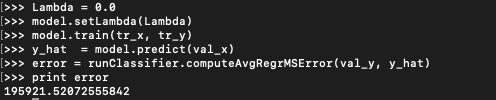
\includegraphics[width=0.3\linewidth]{Ridge regression error when gamma is 0.png}

\end{center}

\caption{Ridge regression error (gamma = 0.0)}

\label{fig:long}

\label{fig:onecol}

\end{figure}

Figure 2 is the graph with x-axis is gamma which sweeps from 0.0 to 1.0 and y-axis is the accuracy of the model. By this figure, we can see that the accuracy gets higher as the gamma increases to 1.0 and also it is proportional.
Also on figure 3, we can find out that when the gamma is set to 0.0, which works the same with the vanila linear regression model, the error(195921.xxx..) is same with the figure 1. From this, gamma works as the regularization to reduce the error and it can be verified because the ridge regression error is 195920.xxx... when gamma is set to 1.0.

REPORT3. Your writing goes here.

REPORT4. I failed to get the error because of the error related to tensorflow.
To improvement its effect, we can add regularizers or change the value of how we quantize $Y(tr_y)$.

REPORT5. We use quantizeY to solve the regression problem by converting it classification problem.

REPORT6. 
\begin{figure}[h] 

\begin{center}


\includegraphics[width=1.0\linewidth]{OLS model in scikit-learn.png}

\end{center}

\caption{error printed by OLS model in scikit-learn }

\label{fig:long}

\label{fig:onecol}

\end{figure}

As you can see on this figure 4, the error from OLS model in scikit-learn(195894.xxx..) is almost the same with the error from the model I implemented on report 1(195921.xxx). The very slight difference can be interpreted by the existence of the bias term. I did not consider the bias term but the scikit-learn model might have considered this.

REPORT7.
\begin{figure}[h] 

\begin{center}

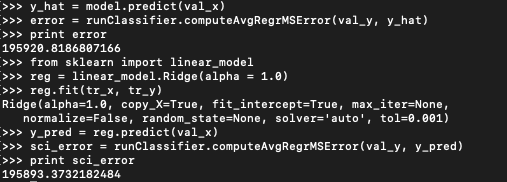
\includegraphics[width=1.0\linewidth]{ridge regression model by myself and by scikit-learn.png}

\end{center}

\caption{error printed by ridge regression I implemented and scikit-learn both }

\label{fig:long}

\label{fig:onecol}

\end{figure}

As you can see on this figure 5, the error from ridge regression model in scikit-learn(195893.xxx..) is almost the same with the error from the model I implemented on report 1(195920.xxx). The very slight difference can be interpreted by the existence of the bias term. I did not consider the bias term but the scikit-learn model might have considered this. It looks like the same situation with the report 6.

REPORT8.
\begin{figure}[h] 

\begin{center}

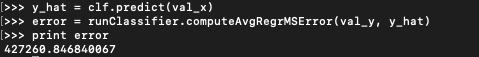
\includegraphics[width=1.0\linewidth]{Logistic regression model in scikit-learn model.png}
\end{center}

\caption{error printed by logistic regression model in scikit-learn model}

\label{fig:long}

\label{fig:onecol}

\end{figure}

On figure 6, the error printed by logistic regression model in scikit-learn model is 427260.xxx... . I could not get the error of the logistic regression model I implemented, but I think when I fix the slight error on my setting it will print the similar error like this figure.

REPORT9.
I used ridge regression that I implemented on kaggle uploaded file as result.csv.
My private score is 205714.19400 and the public score is 223480.70964. 
\end{document}

